% \iffalse meta-comment
%
% Copyright (C) 2024 Aliaume LOPEZ
% --------------------------------
%
% This file may be distributed and/or modified under the
% conditions of the LaTeX Project Public License, either version 1.3c
% of this license or (at your option) any later version.
% The latest version of this license is in:
%
% http://www.latex-project.org/lppl.txt
%
% and version 1.3c or later is part of all distributions of LaTeX
% version 2008-05-04 or later.
%
% \fi
%
% \iffalse
%
%<*driver>
\documentclass{ltxdoc}
\usepackage{tikz}
\usepackage{ensps-colorscheme}
\EnableCrossrefs
\CodelineIndex
\RecordChanges
\begin{document}
\DocInput{ensps-colorscheme.dtx}
\end{document}
%</driver>
% \fi
%
%
% \changes{v0.0.1}{2024-05-28}{Initial version}
% \GetFileInfo{ensps-colorscheme.sty}
% \DoNotIndex{\#,\$,\%,\&,\@,\\,\{,\},\^,\_,\~,\ }
% \DoNotIndex{\@ne}
% \DoNotIndex{\advance,\begingroup,\catcode,\closein}
% \DoNotIndex{\closeout,\day,\def,\edef,\else,\empty,\endgroup}
% \DoNotIndex{\foreach,\subitem,\hue,\letter,\hdclindex}
% \DoNotIndex{\begin,\colorlet,\definecolor,\intensity,\end,\shade}
% \DoNotIndex{\y,\x,\xglobal,\newcommand,\name,\node,\variant}
% \title{The \textsf{ensps-colorscheme} package
%    \thanks{This document corresponds to \textsf{ensps-colorscheme}~\fileversion,
%    dated \filedate.}
%}
%\author{Aliaume Lopez \\ \texttt{ad.lopez@uw.edu.pl}}
%
% \maketitle
% \begin{abstract}
%   A simple package to provide the ENS Paris-Saclay colors and theme.
%   It has been reversed engineered from the official Université Paris-Saclay
%   ``Charte Graphique".
% \end{abstract}
%
% \section{Introduction}
%
% This package provides the ENS Paris-Saclay colors and theme.
% It can be used in PhD theses, presentations and other documents
% to ensure a consistent look and feel.
% The package is loosely based on the following document 
%   \texttt{Charte Graphique}\footnote{\url{https://www.universite-paris-saclay.fr/sites/default/files/2020-06/Charte-graphique-UniversiteParisSaclay.pdf}.}.
% 
% For now, the package only provides colors and a way to visualize them.
%
% \section{Usage}
% The package defines the following colors:
% \begin{itemize}
%   \foreach \name in {A,B,C,D} {
%       \foreach \hue in {1,2,3,4,5} {
%           \item \texttt{\name\hue}:
%               \textcolor{\name\hue}{\rule{0.5em}{0.5em}}
%               (respectively \texttt{\name\hue bg}
%                \textcolor{\name\hue bg}{\rule{0.5em}{0.5em}} and 
%                \texttt{\name\hue hint}
%                \textcolor{\name\hue hint}{\rule{0.5em}{0.5em}})
%       }
%   }
%   \item \texttt{Prune}:
%       \textcolor{Prune}{Prune}
% \end{itemize}
%
% \DescribeMacro{\enspscolors}
% The \cs{enspscolors} command creates a small tikzpicture with the ENS Paris-Saclay colors.
% Producing the following output:
% \begin{center}
%     \enspscolors
% \end{center}
%
% \PrintIndex
% \PrintChanges
%
% \section{Implementation}
%
% Here we define the colors for the ENS Paris-Saclay theme.
% The main colors are hard coded, and the \texttt{bg} and \texttt{hint} colors
% are then computed from the main colors.
%    \begin{macrocode}
\NeedsTeXFormat{LaTeX2e}[2023-11-01] 
\ProvidesPackage{ensps-colorscheme}
 [2024-05-03 v0.0.1 ENS Paris-Saclay Colors and Theme]
\RequirePackage{tikz}
\definecolor{Prune}{RGB}{99,0,60}
\definecolor{A1}{HTML}{000000}
\definecolor{B1}{RGB}{49,62,72}
\definecolor{C1}{RGB}{124,135,143}
\definecolor{D1}{RGB}{213,218,223}
\definecolor{A2}{RGB}{198,11,70}
\definecolor{B2}{RGB}{237,20,91}
\definecolor{C2}{RGB}{238,52,35}
\definecolor{D2}{RGB}{243,115,32}
\definecolor{A3}{RGB}{124,42,144}
\definecolor{B3}{RGB}{125,106,175}
\definecolor{C3}{RGB}{198,103,29}
\definecolor{D3}{RGB}{254,188,24}
\definecolor{A4}{RGB}{0,78,125}
\definecolor{B4}{RGB}{14,135,201}
\definecolor{C4}{RGB}{0,148,181}
\definecolor{D4}{RGB}{70,195,210}
\definecolor{A5}{RGB}{0,128,122}
\definecolor{B5}{RGB}{64,183,105}
\definecolor{C5}{RGB}{140,198,62}
\definecolor{D5}{RGB}{213,223,61}
\foreach \name in {A,B,C,D} {
    \foreach \hue in {1,2,3,4,5} {
        \foreach \shade/\intensity in {hint/20,bg/50} {
            \xglobal\colorlet{\name\hue\shade}{\name\hue!\intensity!white}
        }
    }
}
%    \end{macrocode}
%
% \begin{macro}{\enspscolors}
% Create a small tikzpicture with the ENS Paris-Saclay colors.
%    \begin{macrocode}
\newcommand{\enspscolors}{
    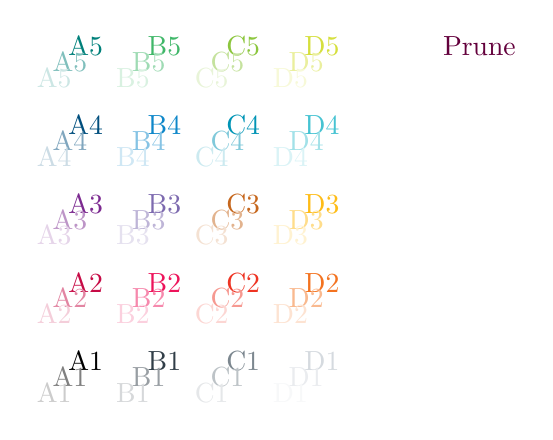
\begin{tikzpicture}
        \foreach \letter/\x in {A/0,B/1,C/2,D/3} {
            \foreach \y/\variant in {0/1,1/2,2/3,3/4,4/5} {
                \node[color=\letter\variant] 
                    (\letter\variant) at (\x,\y) 
                    {\letter\variant};
                \node[color=\letter\variant bg]
                    (BG\letter\variant) at ({\x - 0.2}, {\y - 0.2}) 
                    {\letter\variant};
                \node[color=\letter\variant hint] 
                    (HT\letter\variant) at ({\x - 0.4}, {\y - 0.4}) 
                    {\letter\variant};
            }
        }
        \begin{scope}[xshift=2cm]
            \foreach \name/\x/\y in {
                Prune/3/4
            } {
                \node[color=\name] (\name) at (\x,\y) 
                     {\name};
            }

        \end{scope}
    \end{tikzpicture}
}
%    \end{macrocode}
% \end{macro}
%
% \Finale
\endinput
